\documentclass[10pt,a4paper]{report}
\usepackage[utf8x]{inputenc}
\usepackage{ucs}
\usepackage{amsmath}
\usepackage{amsfonts}
\usepackage{amssymb}
\usepackage{makeidx}
\usepackage{graphicx}
\usepackage[brazil]{babel}
\usepackage{hyperref}
\usepackage{pdfpages}
\author{Vagner Clementino}
\title{Relatório de Progresso do Mestrado\\
	Vagner Clementino}
	\makeindex

\begin{document}
\maketitle

\chapter{Objetivo do Documento}
\label{sec:objetivo}

O presente documento tem por objetivo subsidiar o pedido de prorrogação de
defesa do aluno Vagner Clementino dos Santos. Ele detalha o histórico da vida
acadêmica do aluno, descreve a situação atual das atividades sendo desenvolvidas
e apresenta um plano de trabalho visando a conclusão da dissertação.  O texto se
dedica ainda em justificar o pedido de prorrogação. Cabe ressaltar que se trata
de um pedido complementar a outro realizado em julho deste ano o qual foi
aprovado por este colegiado.

\chapter{Histórico do Aluno}
\label{sec:historico}

O aluno Vagner Clementino dos Santos ingressou no Programa de Pós Graduação em
Ciência da Computação (PPGCC) no segundo semestre de 2014 sob a orientação do
professor Rodolfo F. Resende. Trata-se de um aluno de tempo parcial que divide o
seu tempo como aluno de mestrado e analista de desenvolvimento na Empresa de
Informática de Belo Horizonte (PRODABEL), onde trabalha 40 horas semanais.

O período 2014/2, primeiro semestre como aluno do PPGCC, foi devotado às
disciplinas do programa, sendo que a proposta de dissertação estava sendo
planejada com base na literatura da área. No período 2015/1 a proposta de
dissertação foi materializada e apresentada ao colegiado em maio de 2015. Sob o
título de \textit{UMA LINGUAGEM PARA MODELAGEM CONCEITUAL EM XBRL} foi proposto
o desenvolvimento de uma linguagem conceitual para a XBRL (\textit{eXtensible
	Business Reporting Language})\footnote{\url{www.xbrl.org}} que é uma
linguagem para divulgação e intercâmbio de informações financeiras baseada em
XML\@. O tema foi escolhido por se tratar de um assunto de interesse no contexto
do trabalho do mestrando. Contudo, durante o desenvolvimento da referida
proposta, a conjunção de fatores que a sustentavam deixou de existir, sendo
necessária a apresentação de um novo projeto de dissertação.

Em dezembro de 2015 foi apresentada uma nova proposta denominada  \textit{UM
	ESTUDO DE FERRAMENTAS DE SUPORTE DE PROBLEMAS DE SOFTWARE (FSPS)} que, em
síntese, visa investigar e contribuir na questão de como este tipo de ferramenta
vem sendo melhorada ou estendida no contexto da transformação do processo de
desenvolvimento de software, bem como da manutenção, de um modelo tradicional
para um outro que incorpora práticas ágeis. As Ferramentas de Suporte de
Problemas de Software são aquelas utilizadas pelas organizações para
\textit{gerenciar as Requisições de Mudança}\cite{1703974} em Software.

A proposta sobre as FSPS's encontra-se em desenvolvimento e foi revista após
análise do colegiado ocorrida em junho/2016. Após realizada as adequações
solicitadas pelo revisor, o documento foi apresentado ao colegiado em 03/07/2016
e encontra-se em análise. Não obstante, as tarefas relativas à dissertação desde
então continuam sendo realizadas. Tais atividades estão detalhadas na
Capítulo~\ref{situacao-atual}.

Os créditos necessários à integralização do curso já foram obtidos faltando
apenas aqueles relativos à Elaboração de Trabalho Final conforme disposto na
Tabela~\ref{tab:historico}. Conforme orientado no parecer do pedido de
prorrogação realizado anteriormente, este semestre está dedicado unicamente à
elaboração do trabalho final.

\begin{table}[htb]
	\centering
	\begin{tabular}{llllllll}
		\hline
		Período & Turma         & Nome Atividade                           &
		Nota & Conceito & Sit. Final & Créditos & Integralizado \\ \hline
		2014/2  & DIP DCC831PG9 & TÓPICOS ESPECIAIS EM CIÊNCIA DA COMPUTAÇÃO & 80
		& B    & A         & 4        & Sim           \\
		2014/2  & DIP DCC890PG  & TÓPICOS EM ENGENHARIA DE SOFTWARE        & 91
		& A    & A         & 4        & Sim           \\
		2015/1  & DIP DCC865PG  & PROJETO E ANALISE DE ALGORITMOS          & 70
		& C    & A         & 4        & Sim           \\
		2015/1  & DIP DCC890PG2 & TÓPICOS EM ENGENHARIA DE SOFTWARE        & 73
		& C    & A         & 4        & Sim           \\
		2015/2  & DIP DCC890PG1 & TÓPICOS EM ENGENHARIA DE SOFTWARE        & 81
		& B    & A         & 4        & Sim           \\
		2016/1  & DIP DCC890PG1 & TÓPICOS EM ENGENHARIA DE SOFTWARE        & 60
		& D    & A         & 4        & Sim           \\
		2016/1  & DIP DCC904PG  & ESTAGIO EM DOCÊNCIA I                    & 97
		& A    & A         & 2        & Sim           \\
		2016/1  & ETF GER000    & ELABORAÇÃO DE TRABALHO FINAL             &
		&      &           & 0        & Sim           \\
		2016/2  & ETF GER000    & ELABORAÇÃO DE TRABALHO FINAL             &
		&      &           & 0        & Sim           \\ \hline
	\end{tabular}
	\caption{Histórico Escolar Aluno}\label{tab:historico}
\end{table}

\chapter{Situação Atual do Trabalho}
\label{situacao-atual}

O trabalho de dissertação encontra-se em andamento e é composto pelas atividades
listadas a seguir.

\begin{itemize}
	\item Mapeamento Sistemático da Literatura~\cite{keele2007guidelines}
	\item Caracterização das Ferramentas de Suporte de Problemas de Software
		(FSPS)
	\item Pesquisa (Survey) com os
		desenvolvedores~\cite{wohlin2012experimentation}
\end{itemize}

Em comparação ao pedido apresentado ao colegiado em julho deste ano é possível
observar que a atividade ``Desenvolvimento de extensões para as FSPS's'' foi
removida. Esta ação ocorreu para adequação ao cronograma  anteriormente
previsto, no qual a defesa ocorrerá em janeiro/2017. Neste caso, o
desenvolvimento de extensões estaria no escopo dos trabalhos futuros deste
estudo.

Nas próximas subseções é detalhado o andamento de cada etapa deste trabalho de
dissertação. Um resumo de cada atividade desenvolvida pode ser visualizado na
Tabela~\ref{tab:situacao}

\begin{table}[ht]
	\centering
	\resizebox{\textwidth}{!}{%
		\begin{tabular}{|c|l|c|}
			\hline
			\textbf{\#} & \multicolumn{1}{c|}{\textbf{Descrição}}                                                                                                      & \textbf{Situação}  \\ \hline
			01          & Caracterização dos Sistemas de Controle de Demandas
			com base nos requisitos comum a todos eles
				& Em desenvolvimento\\ \hline
			02          & Mapeamento das propostas de extensões existente na literatura                                                                                & Feito  \\ \hline
			03          & Coleta da opinião (survey)dos profissionais & Em Desenvolvimento \\ \hline
		\end{tabular}%
	}
	\caption{Situação das Atividades da Dissertação}
	\label{tab:situacao}
\end{table}


\subsection{Mapeamento Sistemático da Literatura}
\label{subsec:revisao_sistematica}

Um \textit{Mapeamento Sistemático da Literatura}, também conhecido como Estudos
de Escopo (Scoping Studies), tem como objetivo fornecer uma visão geral de
determinada área de pesquisa, estabelecer se existem evidências de estudos sobre
determinado tema e fornecer uma indicação da quantidade de trabalho na linha de
pesquisa sob análise \cite{keele2007guidelines,wohlin2012experimentation}. Esta
etapa do trabalho foi finalizada e os seus resultados estão sendo utilizados
para o planejamento do survey com os profissionais (vide Subseção
\ref{subsec:survey} ).

\subsection{Caracterização das funcionalidades das Ferramentas de Suporte de Problemas de Software }
\label{subsec:caracterizacao}

Esta etapa do trabalho consiste de um estudo exploratório com o objetivo de
determinar quais são as funcionalidades comuns às Ferramentas de Suporte de
Problemas de Software (FSPS). O estudo será feito com base na leitura da
documentação de algumas FSPS para que de forma sistemática seja levantado quais
são as funcionalidades oferecidas por determinada ferramenta. As ferramentas
foram escolhidas mediante uma pesquisa (survey) com profissionais envolvidos em
manutenção de software. A escolha se deu com base em uma lista disponível na
Wikipédia que compara diversas
FSPS\footnote{\url{https://en.wikipedia.org/wiki/Comparison_of_issue-tracking_systems}}.

A previsão que esta etapa esteja finalizada na primeira semana de novembro/2016.
O resultado deste estudo permite compreender melhor este tipo de ferramenta
tomando como base as suas funcionalidades em comum. Também é possível propor
uma taxonomia para as FSPS tendo em vista a possibilidade de determinar o
conjunto mínimo de funções deste tipo de sistema. Uma outra utilização dos
resultados desta etapa consiste no planejamento e desenvolvimento de um survey
com profissionais envolvidos em manutenção de software.

\subsection{Pesquisa com Profissionais}
\label{subsec:survey}
Com o objetivo de coletar os aspectos mais importantes das FSPS's do ponto de
vista dos profissionais ligados à manutenção de software será realizada uma
pesquisa (survey). O planejamento e o desenho da pesquisa seguirá as diretrizes
propostas em \cite{wohlin2012experimentation}.

As etapas de planejamento e desenho do survey  estão sendo realizadas em
conjunto com as outras descritas anteriormente. Neste sentido a previsão que os
dados da pesquisa estejam disponível ao final da segunda semana de
novembro/2016.

Cabe ressaltar que a estratégia utilizada neste estudo é de escrever o texto de
cada uma daquelas atividades no momento de execução das mesmas. Neste sentido,
quando uma parte do trabalho está finalizada cabe apenas redigir as etapas de
resultado e discussão tendo em vista que as demais partes já foram escritas
cabendo apenas revisões pontuais.

\chapter{Justificativa do Pedido}
\label{justificativa}

A prorrogação de defesa deste trabalho de dissertação é realizada com seguintes argumentos:

\begin{itemize}
	\item Sou aluno de tempo parcial e apenas nos últimos seis meses foi
		possível reduzir a minha carga horária de trabalho para 06 horas.
		Antes, todavia, cumpria 40 semanais. Desta forma, a primeira parte do
		mestrado dediquei o meu tempo as disciplinas do curso. 
	\item  Na primeira proposta de dissertação, que tratava de uma linguagem
		\texttt{'XML-LIKE'} denominada XBRL, verifiquei que o tema não tinha
		conexões com meus objetivos profissionais e escopo de trabalho.
		Naturalmente esta mudança no tema resultou em atrasos na realização da
		dissertação, contudo, foi importante por me dar a oportunidade de
		trabalhar com algo mais próximo dos meus objetivos profissionais.
	\item Efetuei uma nova proposta que foi submetida para análise em
		dezembro/2015 e foi parcialmente aceita em junho/2016, sendo necessário
		alguns ajustes.
	\item Houve um pedido realizado em julho/2016 em que o parecer foi favorável
		a defesa ser realizada a partir de janeiro/2017 por conta da situação do
		trabalho na data do pedido bem como pelas atividades propostas. Não
		obstante, a liberação realizada pelo colegiado é de no máximo 90 dias
		tendo o aluno a possibilidade de solicitar um novo pedido de mesmo
		prazo.
\end{itemize}

Com base nos argumentos expostos solicito a este colegiado a prorrogação da
minha defesa. Conforme exposto trata-se de um segundo pedido que visa
complementar aquele realizando em julho/2017. No primeiro pedido foi solicitada
a prorrogação até janeiro/2017, contudo, o colegiado apenas pode deliberar por
90 dias, cabendo ao aluno realizar um novo pedido de mesmo prazo caso assim
julgue necessário. O trabalho se encaminha para finalização podendo ser
apresentado antes do prazo solicitado. Estou sempre à disposição para
esclarecimentos.

\chapter{Plano de Trabalho}
\label{Plano_de_Trabalho}
 As atividades para atingir o objetivo da dissertação são exibidas a seguir mediante um Cronograma e o Quadro de Detalhamento das Atividades da Dissertação. 

 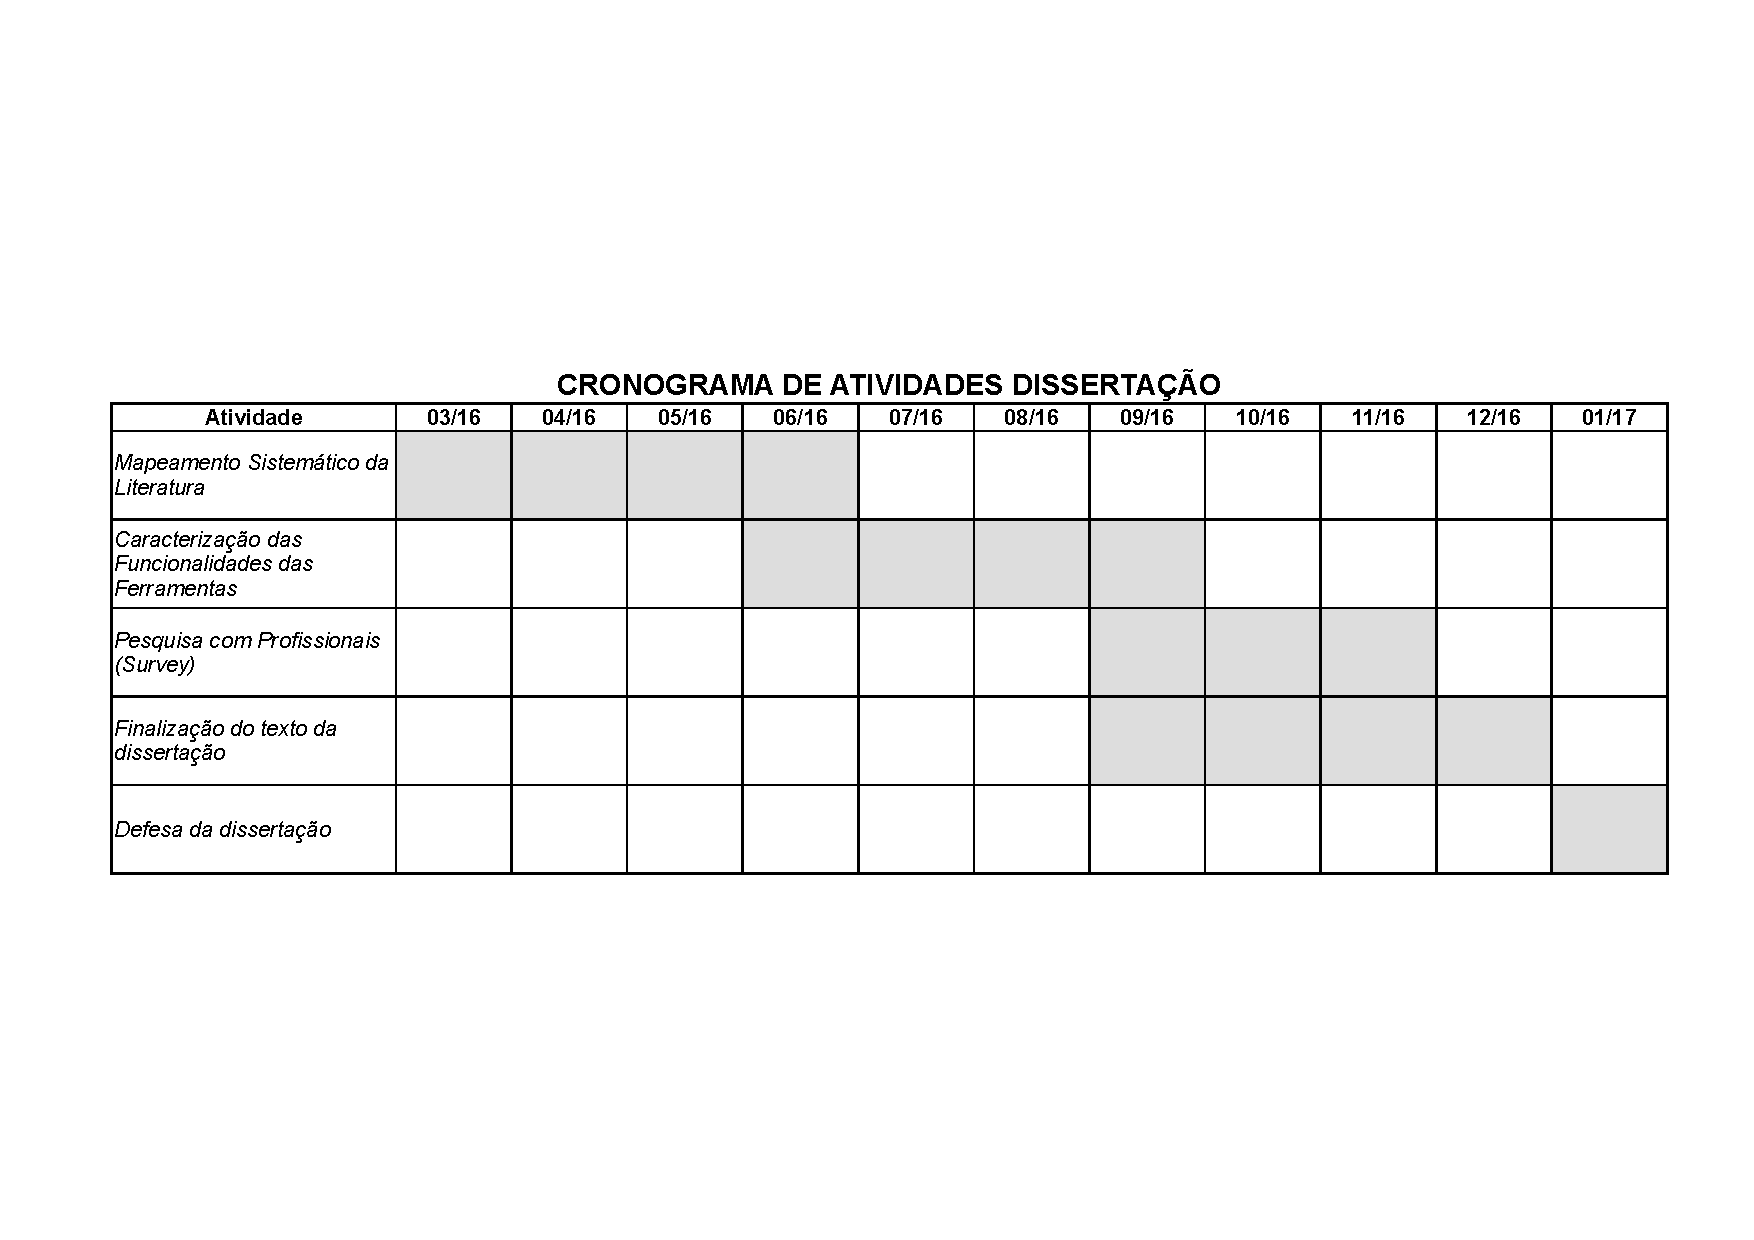
\includepdf{Cronograma-Atividades-Dissertacao.pdf}
 
 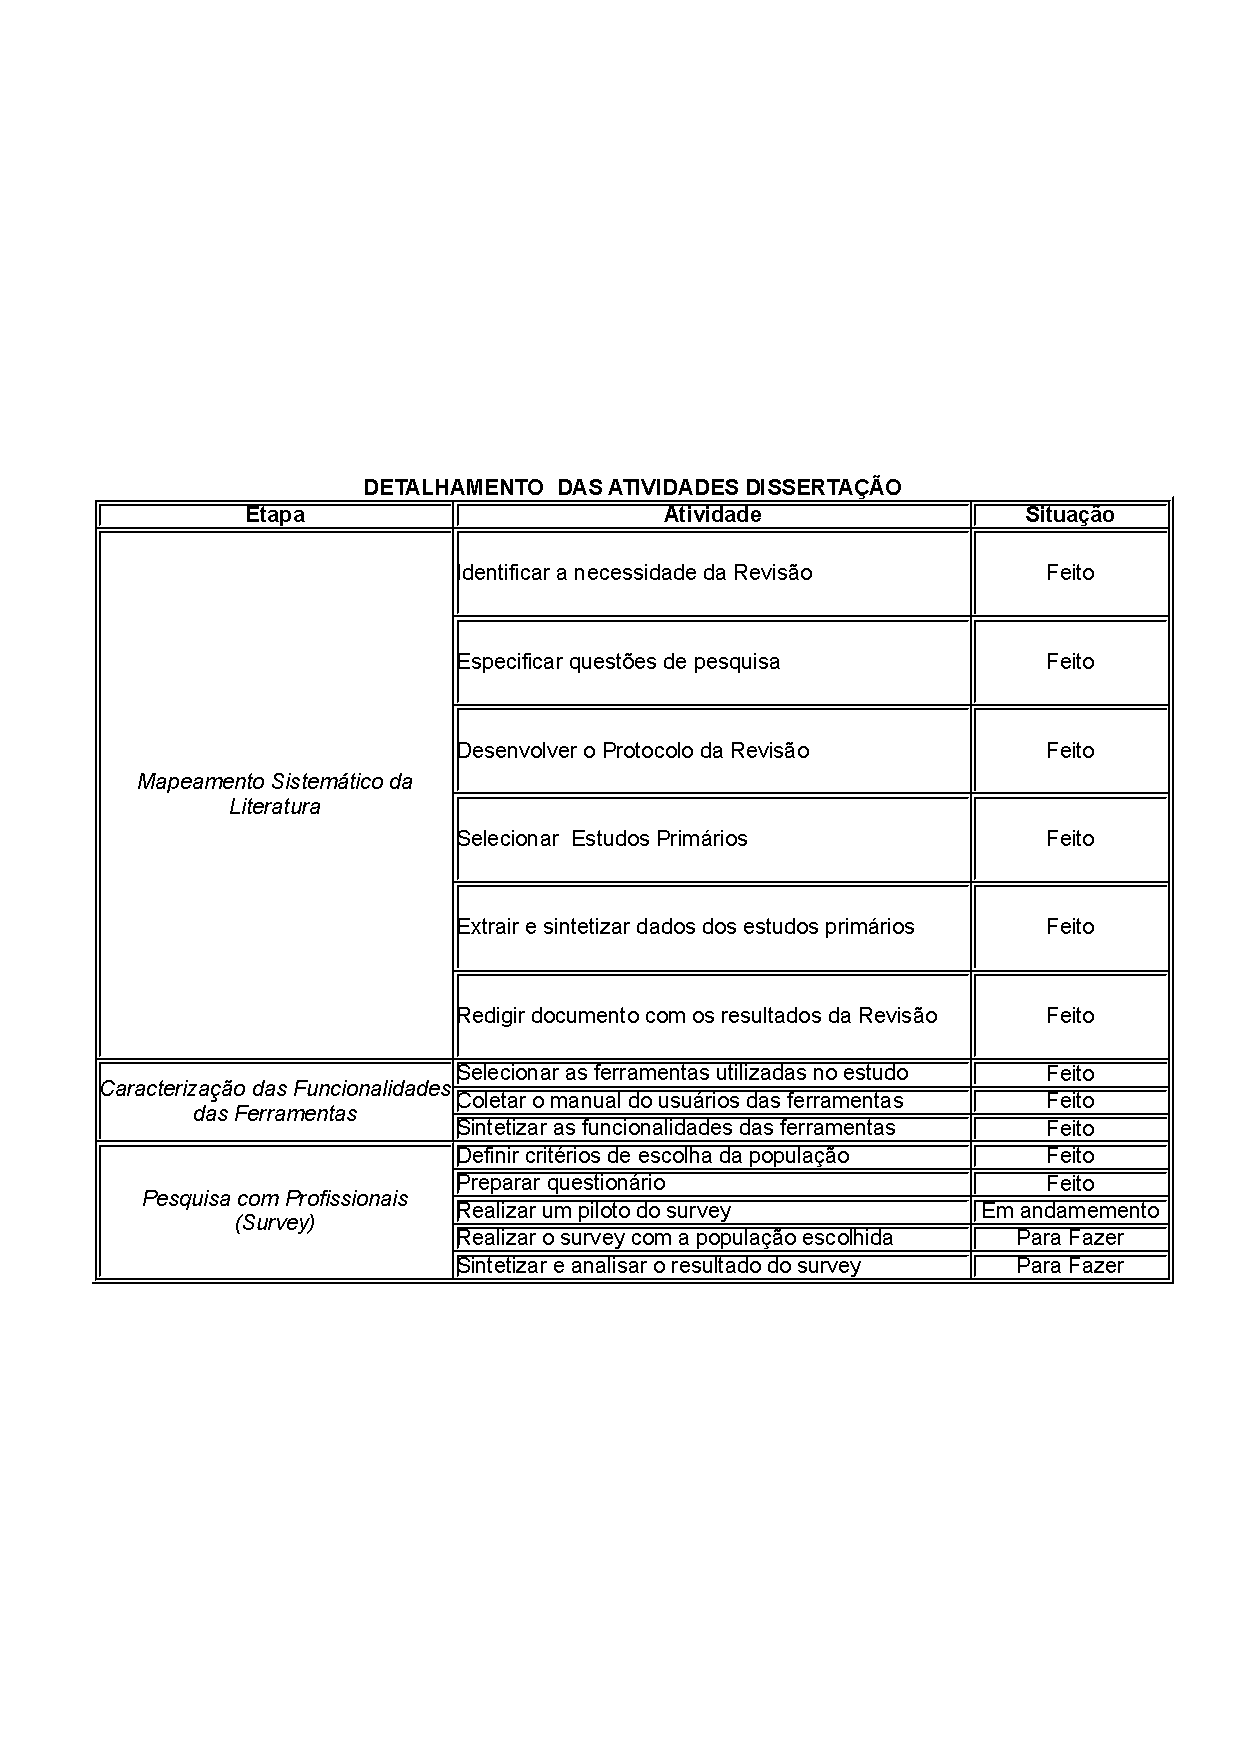
\includepdf{Detalhamento-Atividades-Dissertacao.pdf}

\bibliographystyle{acm}
\bibliography{relatorio}
\end{document}